\href{http://player.vimeo.com/video/15880455}{Shelly Terrell, Global
Netweaver, Curator, PLN Builder} \textbf{} \textbf{Summary}

A. PLNs are the collections of people and information resources (and
relationships with them) that people cultivate in order to form their
own learning networks -- living, growing, responsive sourcses of
information, support, and inspiration that support self-learners..

1. PLNs can be as simple or complex as you would like to make them;
using dashboards like \href{http://www.netvibes.com/en}{Netvibes}, RSS
feeders like \href{http://www.google.com/reader}{Google Reader},
Bookmarking services like \href{http://www.diigo.com/}{Diigo},
\href{https://posterous.com/}{Posterous}, and
\href{http://delicious.com/}{Delicious}, curating with services like
\href{http://www.scoop.it/}{Scoop.it},
\href{http://www.pearltrees.com/}{Pearltrees}, or
\href{http://www.curated.by/}{curated.by}, and finding people and sites
of interest to you via Twitter, Facebook, Google+, and others.

2. Once you've put them together you have a connection of people,
places, and data that allow you to learn, share and make the most of
what's out on the Web that is relevant to you. Learning how to do that
is key.

Introducing
\href{http://dmlcentral.net/blog/howard-rheingold/shelly-terrell-global-netweaver-curator-pln-builder}{his
interview with PLN expert Shelly Terrell}, Howard Rheingold describes
his experience:

``When I started using social media in the classroom, I looked for and
began to learn from more experienced educators. First, I read and then
tried to comment usefully on their blog posts and tweets. When I began
to understand who knew what in the world of social media in education, I
narrowed my focus to the most knowledgeable and adventurous among them.
I paid attention to the people the savviest social media educators paid
attention to. I added and subtracted voices from my attention network,
listened and followed, then commented and opened conversations. When I
found something I thought would interest the friends and strangers I was
learning from, I passed along my own learning through my blogs and
Twitterstream. I asked questions, asked for help, and eventually started
providing answers and assistance to those who seemed to know less than
I. The teachers I had been learning from had a name for what I was doing
--''growing a personal learning network." So I started looking for and
learning from people who talked about HOW to grow a ``PLN'' as the
enthusiasts called them."

\textbf{II. Mindmap for PLNs}
http://dmlcentral.net/blog/howard-rheingold/shelly-terrell-global-netweaver-curator-pln-builder
\textbf{III. Cultivating your garden} A. Howard Rheingold's notes on
\href{http://howardrheingoldsteachingnotes.posterous.com/notes-on-growing-a-personal-learning-network}{cultivating
a PLN}

\begin{center}
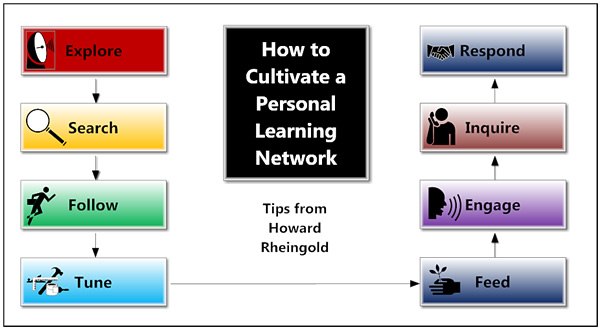
\includegraphics[width=.75\textwidth]{./pictures/network.jpg}
\end{center}

B. Strong and weak ties

1. Your PLN will have people and sites that you check on often - your
main sources of information and learning - your `strong ties'. Your
`weak ties' are those people and sites that you don't allow a lot of
bandwidth or time. But they may become strong over time, as your network
grows or your interests expand.

2. This is a two-way street - it is very important that you are sharing
what you learn and discover with those in your network and not just
taking, if you want to see your network expand.

III. Articles and References

\begin{itemize}
\item
  George Siemens
  \href{http://www.itdl.org/journal/jan\_05/article01.htm}{Connectivism:
  A learning theory for the digital age}
\item
  \href{http://dmlcentral.net/blog/howard-rheingold/shelly-terrell-global-netweaver-curator-pln-builder}{Shelly
  Terrell: Global Netweaver, Curator, PLN Builder} blog post, video
\item
  Will Richardson and Rob Mancabelli,
  \href{http://weblogg-ed.com/2011/personal-learning-networks-an-excerpt/}{Personal
  Learning Networks: Using the Power of Connection to Transform
  Education}
\item
  \href{http://en.wikipedia.org/wiki/Heutagogy}{Heutagogy} - The study
  of self-determined learning
\item
  \href{http://delicious.com/hrheingold/pln}{Howard Rheingold's PLN
  links}
\item
  Links to other articles in ths handbook:
  \href{http://peeragogy.org/connectivism-in-practice-how-to-organize-a-mooc/}{Connectivism
  in practice: How to MOOC,} Personal Learning Plans
\end{itemize}
\subsection{\href{http://socialmediaclassroom.com/host/peeragogy/wiki/initial-outline-source-book}{Return
to Handbook Outline}}

